
\documentclass[conference]{IEEEtran}
\usepackage{graphicx,booktabs,array,url}

\begin{document}

\title{Electronics, Sensors and System Architecture of an Autonomous Search-and-Rescue Quadcopter}
\author{\IEEEauthorblockN{Yuvvraj Kalra}
\IEEEauthorblockA{Manipal Institute of Technology\\Manipal, India\\yuvvrajkalra60@gmail.com}}
\maketitle

\begin{abstract}

The following report covers the analysis of an Autonomous Search and Rescue Quadcopter drone. In this report, I have suggested an architecture comprising of the following components - Pixhawk 6C running ArduPilot as the flight controller, Jetson Orin Nano as companion computer, u-blox M9N GNSS with compass(F9P for RTK) for positioning, Intel RealSense D435 for obstacle detection, RGB + thermal camera running YOLO for human detection, 915/433MHz telemetry radio for communication, and RC, Wi-Fi/4G for audio and video communications. 
\end{abstract}

\begin{IEEEkeywords}
UAV, flight controller, MAVLink, sensors, companion computer, search and rescue
\end{IEEEkeywords}

\section{Introduction}
Search and Rescue is a task that goes beyond the regular importance of success and failure in missions, it involves the lives of our fellow human beings. Thus in such tasks where the acceptable error rate should be 0, we cannot rely on solely human operated machinery, a more efficient system is needed for such precise tasks. Autonomous drones therefore fulfill this need, they accomplish tasks with great precision, their thermal sensor detect life more accurately than humans can, and therefore offer a solution to this dilemma. This report covers one such drone, it goes through its various components as well as the role and significance of each component.


\section{Drone System Overview}
A multirotor consists of a flight controller (FC), electronic speed controllers (ESCs), brushless motors with propellers, a battery with power distribution, GPS, an RC receiver, a telemetry radio, sensors, an optional companion computer, and a ground control station (GCS). Furthermore the attached diagram shows this structure.\cite{ardupilot}.

\section{Electronic Components}
\subsection{Flight Controller}
Principle: A flight controller is an embedded electronics system responsible for controlling the flight of the drone. It is responsible for stabilization, and uses the data taken by the IMU, Magnetometer, Barometer, Lidar, and various other sensors to calculate the required response and then send that response to the ESC.
 It is different from the firmware like Ardupilot or PX4, as it is a hardware component rather than the firmware itself(ArduPilot, PX4) \cite{ardupilot,px4}.

\subsection{Electronic Speed Controller}
The Electronic Speed Controller is the electronic power circuit that determines the power delivered to the brush-less motors of the drone. The flight controller sends a signal directly to Electronic Speed Controller which then switches power to the motors in the required sequence to perform the action. The Electronic Speed Controller does not actually decide what the drones motors are supposed to do, rather it simply recieves commands from the flight controller and sends power as per that command.


\subsection{Brushless Motors and Propellers}
This drone design uses Brushless motors, these motors use electric commutations rather than mechanical brushes. It consists of Stators and Rotators. A Stator is a stationary coil that when energised by the Electronic Speed Controller, generates a magnetic field which causes a torque, thus making the Rotors - the spinning part containing permanent magnets- spin.
Propellers, on the other hand, are the shaped blades on a drone. Which, when spun, generate a thrust, the direction of the thrust depending on the motion of the blades. The Propellers are attached to the Rotors of the drone.
A KV rating determines the RPM of the motor per unit of voltage delivered to it, and is thus a useful metric to look at when choosing a motor. 


\subsection{Battery and Power System}
LiPo and Li-ion batteries are both batteries often used in drones. LiPo batteries provide faster currents, and are more suited to be used in cases like a multi rotor drone which may need rapid changes in motor power.
On the other hand, Li-ion batteries offer higher energy density and thus are used for higher flight durations.
Some important terms:
S-count : This determines the number of batteries connected in series. eg, if a typical cell provides 4V, a 4S of that cell would provide 16V.
Battery capacity : Determines how much charge in mAh the battery can hold.
C Rating : Determines the actual discharge capabilities of the battery, ie, the safe speed it can discharge or charge with respect to its total charge. 
C-rate = Current / Capacity

\subsection{GPS and GNSS}
Global Navigation Satellite Systems are systems which are used to find the location of objects using satellite signals, GPS is one such system created by the USA. The location is estimated by measuring the distance of the receiver from various satellites, this estimation is expressed in terms of longitude, latitude and altitude, this process is also known as trilateration. 
RTK GNSS, or Real Time Kinetic GNSS further improves accuracy by using correctional data to reduce satellite positional errors, in optimal conditions it can even provide centimeter accuracy. The correctional data used by RTK can be provided by a local base station or an online tool like NTRIP.
\begin{table}[h]
\centering\caption{Standard GNSS vs RTK}
\begin{tabular}{lll}\toprule
 & Standard GNSS & RTK GNSS\\\midrule
Accuracy & Typically 2–5 metres\\& under favourable conditions & Centimetre-level \\&&under suitable conditions\\
Needs & GNSS receiver \\  &  and satellite signals & RTK-capable receiver\\ &and correction data \\&(base station/NTRIP)\\
Cost & Generally lower & Generally higher.\\\bottomrule
\end{tabular}
\end{table}

\subsection{RC Transmitter and Receiver}
Radio Control Transmitter is the device used by the pilot to send instructions to the drone, while the Receiver is the device that receives these instructions and passed them to the flight controller.
This device often uses multiple channels to transmit control inputs, the commands it recieves are usually throttle, roll, pitch, and yaw. The additional switches can also be used as arm/disarm switch, flight modes, or for other auxiliary functions.
ELRS, or ExpressLRS is an open source radio channel system that works to provide low latency, responsive control over long ranges.
A failsafe is the drones set response for when the RC signal is lost by that drone, the drone may hold position, land or return to home depending on the selected failsafe.

\subsection{Companion Computer}
A Companion Computer is an additional onboard computer used tasks that exceed the flight controllers computational limits.
It does not share the same tasks as a flight controller, it does not help in stabalisation or motor control. Rather it handles specialised tasks such as image processing, path planning, obstacle detection, and analysis of sensory data. A Raspberry Pi is generally used for such tasks as it is suitable for general purpose computing, but an NVIDIA Jetson may be used in the case of a applications requiring GPU acceleration.
MAVLink is a very basic messaging protocol used by the computer to exchange commands, telemetry, and mission information.

\section{Sensors}
\subsection{IMU}
The Inertiial Measurement Unit is a device that measures the drones movement with an Accelerometer and a Gyroscope. The Accelerometer measures the acceleration of the drone along the 3 axes using specefic force, but it is affected by vibration and drone movement. The Gyroscope measures the rotational motion of the drone and responds appropriately, however it accumulates errors overtime causing drift.

\subsection{Magnetometer}
The Magnetometer used the surrounding magnetic field to get a reference of where the drone is headed with respect to the Earths magnetic north. It can be used alongside other tools to improve orientation estimation and support navigation of the drone. However these readings can be disturbed by the many sources of magnetic interference in the drone, therefore proper sensor placement, calibration, and interference management are needed for its use.

\subsection{Barometer}
The Barometer is a device that measures the atmospheric pressure. This is useful, bacause, as the altitude of the drone rises. the atmospheric pressure decreases, thus it can be used with other metrics to make the altitude data more accurate. This devices meaurements can however be affected by the weather, temperature variation, sensor drift and propeller induced airflow, also known as prop wash.

\subsection{LiDAR}
LiDAR is a device that emits laser light and estimates the distance of objects by measuring the time it take for the light to return.
It exists in 3 forms based on use, it can be used one directionally to find distance long one direction, it can be used 2 directionally to produce a set of distance measurements, and it can be used 3 dimensionally to create a 3D representation of the surroundings. Its common uses include, obstacle detection, terrain mapping, altitude measurement, and navigation. Though it is limited by its high expense, high power usage, weight, lack of usage on transparent or reflective surfaces, and strong ambient lighting conditions.

\subsection{Depth Camera}
A depth camera system estimates distance between the camera to the objects in a scene. Common methods include stereo vision, this estimates depth with comparing features captured from different viewpoints, structured light, which projects a known pattern onto the scene and measures depth from distortion in that pattern, and Time of flight, which uses travel time or phase shift of emitted light.
The performance of the system depends on lighting, scene texture and other environmental conditions.
An example of such as system is the Intel RealSense D435, which also uses RGB imagery\cite{realsense}.
\subsection{Optical Flow Sensor}
This system used changes in the scene to estimate motion relative to a surface over time. It uses apparent movement to estimate relative motion, and is used most often in GPS denied environments. It is limited by poor lighting, high altitude, motion blur and other environmental factors.

\begin{table*}[!t]
\centering
\footnotesize
\renewcommand{\arraystretch}{1.15}
\caption{Perception sensor comparison}
\label{tab:perception}
\begin{tabular}{@{}p{2.2cm}p{3.6cm}p{4.4cm}p{6.3cm}@{}}
\toprule
\textbf{Sensor} & \textbf{Output} & \textbf{Strength} & \textbf{Weakness}\\
\midrule
LiDAR & Distance, 2D/3D point clouds & Works in darkness; precise ranging & Expensive; weight and performance vary; transparent surfaces cause errors\\
Depth camera & Depth image, optionally with RGB & Spatial information; obstacle detection & Performance varies with lighting, surface texture and operating range\\
Optical flow & Relative image motion & Indoor navigation and GPS-denied areas & Needs visible surface features and sufficient lighting; does not directly give absolute position\\
\bottomrule
\end{tabular}
\end{table*}
\section{Additional Sensors}

\subsection{Thermal (Infrared) Camera}
Principle: detects long-wave infrared radiation emitted by objects, so warm bodies appear against cooler surroundings. Application: locating people at night or in light vegetation. Advantages: works in darkness, strong human contrast. Limitations: low resolution, cost, cannot see through glass, weak in hot environments. \cite{thermal}
\subsection{mmWave Radar}
Principle: emits radio waves (e.g., 60--77 GHz) and measures reflections for range and velocity. Application: obstacle detection in smoke, fog, dust and rain; vital-sign sensing research. Advantages: robust to weather and lighting. Limitations: low spatial resolution, noisy returns.\cite{mmWave}

\section{Communication Interfaces}
\begin{table}[h]
\centering\caption{Interfaces in a drone system}
\begin{tabular}{p{0.7cm}p{3.6cm}p{3cm}}\toprule
Interface & Typical use & Example device\\\midrule
UART & Serial point-to-point link & GPS, telemetry radio, companion computer (MAVLink)\\
I2C & Short-range multi-device bus for low-rate sensors & External compass, barometer\\
SPI & Fast sensor bus & Onboard IMU, SD card, OSD chip\\
CAN & Robust multi-node bus & DroneCAN GPS, smart ESCs\\
PWM & Pulse-width control signal & Servos, legacy ESC signal\\
USB & High-speed host/device link & Jetson to FC, USB camera\\\bottomrule
\end{tabular}
\end{table}

\section{System Architecture}
Fig.~\ref{fig:arch} shows the proposed architecture. 1. Power Flow

    Battery: Powers the distribution system, which feeds the ESCs and motors.

    BEC / Regulated Supply: Steps down voltage for the flight controller and electronics.

    Companion Computer \& Sensors: Powered via dedicated supplies matched to their voltage and current needs.

2. Control-Command Flow
    Manual Control: The pilot uses an RC transmitter/receiver to send inputs to the flight controller, which runs stabilization algorithms and commands the ESCs to drive the motors.
    Autonomous Control: The flight controller executes waypoint missions or navigation commands provided by the companion computer.
3. Sensor-Data Flow
    Flight Sensors: The IMU, magnetometer, barometer, and GNSS supply motion, heading, altitude, and position data to the flight controller.
    Environmental Sensors: Depth cameras, LiDAR, and optical flow sensors add spatial awareness.
    Companion Computer: Processes heavy data (e.g., camera feeds) for obstacle/person detection and sends navigation recommendations to the flight controller.
4. Telemetry Flow
    Flight Controller: Relays flight status (battery, position, mode) to the ground station via telemetry.
    Companion Computer: Transmits detection results, images, and mission data to allow operators to monitor the drone and search-and-rescue progress.
\begin{figure*}[t]
\centering
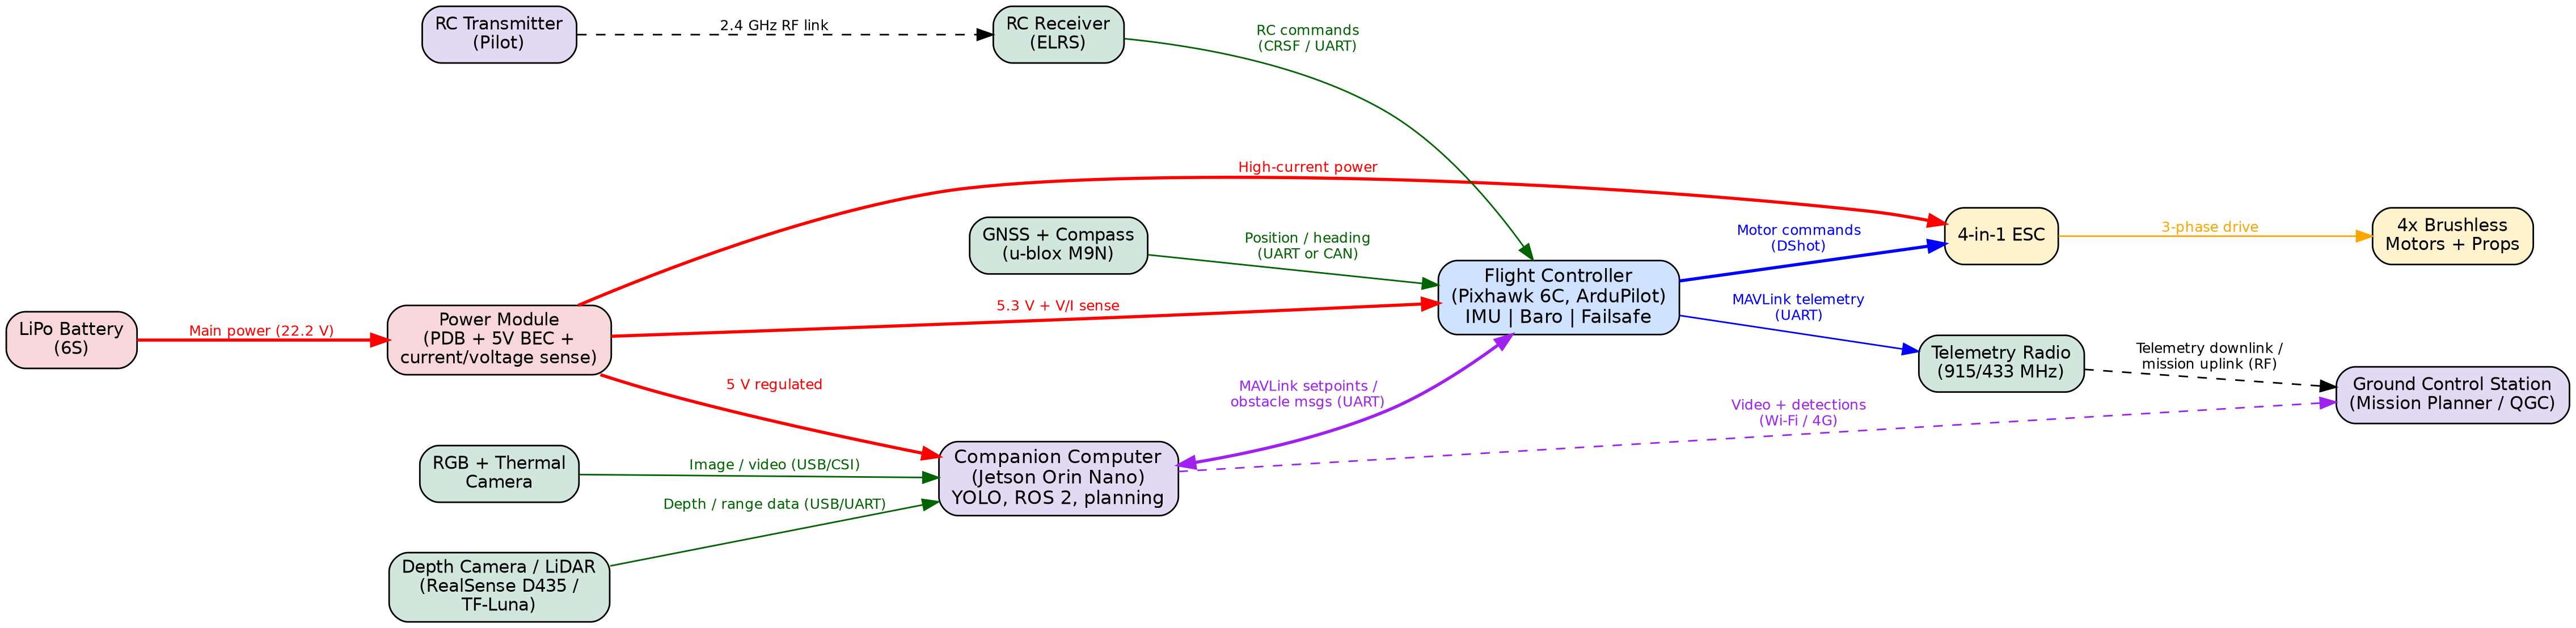
\includegraphics[width=\textwidth]{drone_system_architecture(1).png}
\caption{System architecture of the autonomous search-and-rescue quadcopter.}
\label{fig:arch}
\end{figure*}

\section{Component Selection for Search and Rescue}
\begin{table}[h]
\centering\caption{Selected components}
\begin{tabular}{p{1.6cm}p{2.2cm}p{3.3cm}}\toprule
Function & Choice & Reason\\\midrule
Flight controller & Pixhawk 6C (ArduPilot) & Proven, open firmware, waypoint missions, failsafes, MAVLink, redundant IMUs \cite{pixhawk6c}\\
Companion computer & Jetson Orin Nano & GPU for onboard YOLO and ROS 2, low power versus larger boards \cite{jetson}\\
Positioning & u-blox M9N GNSS + compass (RTK F9P optional) & Reliable outdoor navigation, multi-constellation \cite{ublox}\\
Obstacle sensor & Intel RealSense D435 (or TF-Luna for downward range) & Dense depth in a light package; mature ROS support \cite{realsense}\\
Human detection & RGB + thermal camera with YOLO model & Thermal finds heat signatures at night; RGB confirms detections\\
Communication & 915/433 MHz telemetry radio, ELRS for RC, Wi-Fi/4G for video & Long-range MAVLink link, robust manual override \cite{elrs}\\\bottomrule
\end{tabular}
\end{table}
Flight Controller (Pixhawk 6C + ArduPilot)
    Pros: Redundant IMUs, robust failsafes, ideal for autonomous navigation.
    Trade-offs: Higher weight and cost; requires complex configuration. Cannot process AI workloads.
Companion Computer (NVIDIA Jetson Orin Nano)
    Pros: Onboard GPU acceleration for real-time computer vision, object detection, and ROS 2 processing.
    Trade-offs: Higher power draw, weight, cost, and cooling needs, which can reduce total flight time.
Positioning (u-blox NEO-M9N GNSS; optional ZED-F9P RTK upgrade)
    Pros: NEO-M9N offers reliable, multi-constellation meter-level positioning; ZED-F9P enables centimeter-level precision.
    Trade-offs: RTK setup adds cost, integration complexity, and requires correction data. Both need clear satellite visibility.
Obstacle Sensing (Intel RealSense D435 vs. TF-Luna Rangefinder)
    RealSense D435: Delivers rich 3D depth maps, but demands more processing and is sensitive to lighting and range.
    TF-Luna: Lightweight, simple single-point distance measuring (ideal for downward altitude hold), but lacks full 3D obstacle mapping.
Human Detection (RGB + Thermal Camera with YOLO)
    Pros: Combines visual detail with heat signature detection in darkness using AI models.
    Trade-offs: Increases cost, weight, power draw, and software complexity. Thermal contrast can degrade in warm ambient conditions.
Communication (Telemetry Radio, ELRS Receiver, Wi-Fi / Cellular)
    Setup: Uses telemetry radios (MAVLink data), ELRS (manual pilot override), and cellular/Wi-Fi (high-bandwidth data transfer).
    Trade-offs: Must balance range, power, bandwidth, and local spectrum regulations.

\section{Conclusion}
The design of an autonomous search-and-rescue drone requires the integration of flight-control electronics, power systems, navigation sensors, perception systems, and communication interfaces. The flight controller provides stable flight and failsafe management, while the companion computer enables computationally intensive tasks such as human detection and autonomous path planning. GNSS, LiDAR, depth cameras, optical flow, and thermal imaging provide complementary capabilities, each with limitations under particular environmental conditions. Ultimately, component selection must balance accuracy, reliability, processing capability, payload weight, power consumption, cost, and communication range to achieve safe and effective search-and-rescue operations.

\begin{thebibliography}{99}
\bibitem{ardupilot} ArduPilot Dev Team, ``ArduPilot Documentation,'' [Online]. Available: https://ardupilot.org/copter/. 
\bibitem{px4} PX4 Autopilot, ``PX4 User Guide,'' [Online]. Available: https://docs.px4.io/. 
\bibitem{mavlink} MAVLink Developer Guide, [Online]. Available: https://mavlink.io/en/. 
\bibitem{pixhawk6c} Holybro, ``Pixhawk 6C,'' [Online]. Available: https://docs.holybro.com/.
\bibitem{jetson} NVIDIA, ``Jetson Orin Nano Developer Kit,'' [Online]. Available: https://developer.nvidia.com/embedded/jetson-orin.
\bibitem{ublox} u-blox, ``NEO-M9N / ZED-F9P product pages,'' [Online]. Available: https://www.u-blox.com.
\bibitem{realsense} Intel RealSense, ``Depth Camera D435,'' [Online]. Available: https://www.intelrealsense.com/.
\bibitem{elrs} ExpressLRS, ``ExpressLRS Documentation,'' [Online]. Available: https://www.expresslrs.org/. 
\bibitem{thermal}Thermal Imaging: ''how thermal imaging works''[Online]. Available: https://www.flir.com/discover/professional-tools/how-does-thermal-imaging-work/
\bibitem{mmWave} mmWave radar ''Texas Instruments, mmWave Radar Sensors.''[Online]. Available: https://www.ti.com/sensors/mmwave-radar/overview.html
\end{thebibliography}
\end{document}
